\documentclass[tikz,border=10pt]{standalone}
\usepackage[T1]{fontenc}
\usepackage[utf8]{inputenc}
\usepackage{lmodern}
\usepackage{amsmath,amssymb}
\usetikzlibrary{arrows.meta,positioning,shapes.geometric,calc}
\definecolor{jac}{HTML}{73539E}
\definecolor{ink}{HTML}{354052}
\tikzset{
 >=Stealth,
 state/.style={draw=jac,fill=jac!7,rounded corners=5pt,align=center,minimum width=26mm,minimum height=11mm,inner sep=5pt,font=\small},
 action/.style={state,fill=white},
 decision/.style={draw=jac,fill=jac!7,diamond,aspect=2.4,inner sep=1.8pt,align=center,font=\small},
 success/.style={state,draw=teal!75!black,fill=teal!7},
 failure/.style={state,draw=red!70!black,fill=red!5},
 arrow/.style={->,thick,draw=ink},
 note/.style={align=left,font=\footnotesize,text=ink}
}
\begin{document}

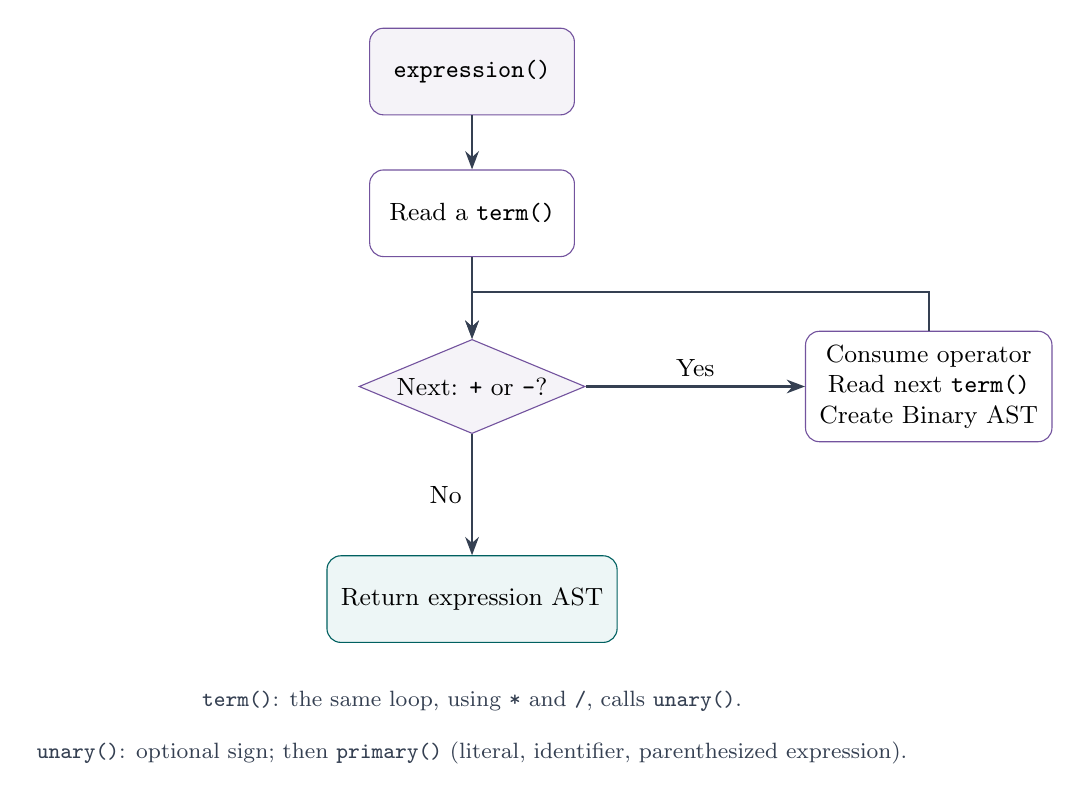
\begin{tikzpicture}[font=\small]
\node[state] (expr) at (0,0) {\texttt{expression()}};
\node[action] (term) at (0,-1.8) {Read a \texttt{term()}};
\node[decision] (add) at (0,-4) {Next: \texttt{+} or \texttt{-}?};
\node[action] (term2) at (5.8,-4) {Consume operator\\Read next \texttt{term()}\\Create Binary AST};
\node[success] (done) at (0,-6.7) {Return expression AST};
\draw[arrow] (expr)--(term);\draw[arrow] (term)--(add);
\draw[arrow] (add)--node[left]{No}(done);
\draw[arrow] (add)--node[above]{Yes}(term2);
\draw[arrow] (term2.north) |- ([yshift=6mm]add.north) -- (add.north);
\node[note] at (0,-8) {\texttt{term()}: the same loop, using \texttt{*} and \texttt{/}, calls \texttt{unary()}.};
\node[note] at (0,-8.65) {\texttt{unary()}: optional sign; then \texttt{primary()} (literal, identifier, parenthesized expression).};
\end{tikzpicture}

\end{document}
